\documentclass{VRARWorkshop}

\usepackage[utf8]{inputenc}
\usepackage[T1]{fontenc}
\usepackage[hidelinks]{hyperref}

\title{Augmented reality for supporting manual non-destructive ultrasonic testing of metal pipes and plates}

%\authors{Robert Deppe, Oliver Nemitz, Jens Herder}
\authors{Anonym}

\affiliations{~}
% TODO: Correct affiliations

\abstract{
The aim of this paper is to describe the application of augmented reality technology in non–destructive testing of products of the metal–industry and a prototype created in the course of a bachelor--thesis.
The prototype is created with hard– and software, that is usually employed in the gaming industry, and delivers positions for creating c–-scans.
Using the ZEDmini in combination with the HTC VIVE enables realtime visualisation of the probes path in the HMD, as well as the setting of virtual markers on the specimen.
As a part of the implementation the downhill–simplex optimization–algorithm is implemented to fit the specimen to a cloud of recorded surfacepoints.
The accuracy is statistically tested and evaluated with the result, that the \textit{VIVE}–trackingsystem is accurate up to ca. 1–-2 millimeters in well set-up conditions.
This paper is of interest not only for research–-institutes of the metal–-industry, but also for any areas of work, in which the enhancement with augmented–reality is possible.
}

% Give some keywords
\keywords{
Nondestructive Testing,
Ultrasonic,
Augmented Reality,
Tracking,
Stereo--camera,
HTC,
ZED,
NDT,
AR
}

\begin{document}

\section{Introduction}

In the field of nondestructive testing of steel products, the ultrasonic (US) inspection is a frequently used method to assure given safety requirements. For heavy plates and large diameter pipes the manual US testing is often applied as a follow-up inspection. Here, a US probe is moved by hand on the surface of the specimen (cf. Figure \ref{fig:manual_UT}). While moving and possibly rotating the probe the operator monitors the US signal on a screen. Usually, in case of an imperfection in the material, the US signal exhibits a higher amplitude and the position of the imperfection can be marked on the specimen.
However, the exact position and orientation of the probe are not captured during the manual inspection. Hence, generating an objective report with for example a map of color coded US amplitudes onto probe positions (C-Scan, cf. Figure fig:cScan) is not directly possible. Furthermore, there is usually no kind of tracking and visualization of those parts of the specimen surface which have already been inspected and especially no control if inspection gaps occur. \\
The aim of our system is therefore to track the position and orientation of the US probe during the inspection and assign them to the corresponding US signals. This tracking is done with standard AR/VR components of an HTC Vive system. Global coordinates of the probe are converted to coordinates in a local coordinate system on the specimen and sent to a UT inspection software which can generate a C-Scan of the inspection. By a ZEDmini stereo camera it is possible to view the inspection in AR and to visualize certain virtual elements as the pathes of the already inspected areas.

Erst Ebene, später Pipe

\begin{figure}[h!]
    \begin{center}
        \includegraphics[width=0.7\textwidth]{images/US-workspace.jpg}
        \caption{\label{fig:manual_UT} Manual ultrasonic testing of steel large diameter pipes.}
    \end{center}
\end{figure}
\begin{figure}[h!]
    \begin{center}
        \includegraphics[width=0.48\textwidth]{images/CScan_Specimen.jpg}
				\hspace{0.5mm}
        \includegraphics[width=0.48\textwidth]{images/CScan_Image.jpg}
        \caption{\label{fig:cScan} A C--Scan is an image where a color-coded amplitudes extracted from the US signal 
				are assigned to positions of the US probe. Here, a rectangular grid with a resolution of 0,1\,mm is used.}
    \end{center}
\end{figure}

\section{Related Research}
\cite{ARPat15}
\cite{ARClean}
\cite{schwerdtfeger_using_2008}
\cite{fadzil_design_2015}
\cite{walter_non-contact_2007}

\section{Basics of non-destructive ultrasonic testing of metal products}

US inspection:
\cite{deutsch_zfp_2010} \\
Phased array (skip?):
\cite{moles_introduction_2004}
\cite{olympus_Grundlagen}

\section{Description of the AR--application}
The AR--application supports manual testing visually, which is connected via an IP connection.
Through a AR-HMD the inspector is able to see the already inspected path and identify gaps.
Position and Rotation is send to the ultrasonic scanning computer, where the data is combined with the measurements received by the probe into a C--Scan.

\section{Implementation}
%and sends the position- and rotationdata to the ultrasonnic scanning computer
The application was implemented in the game--engine Unity.
Attached to the HMD is the \textit{ZEDmini}, a stereo--camera that can be used to display a camera image in the HMD and to create a depth mask.

\cite{dorner_virtual_2013}

\begin{figure}[h!]
    \begin{center}
        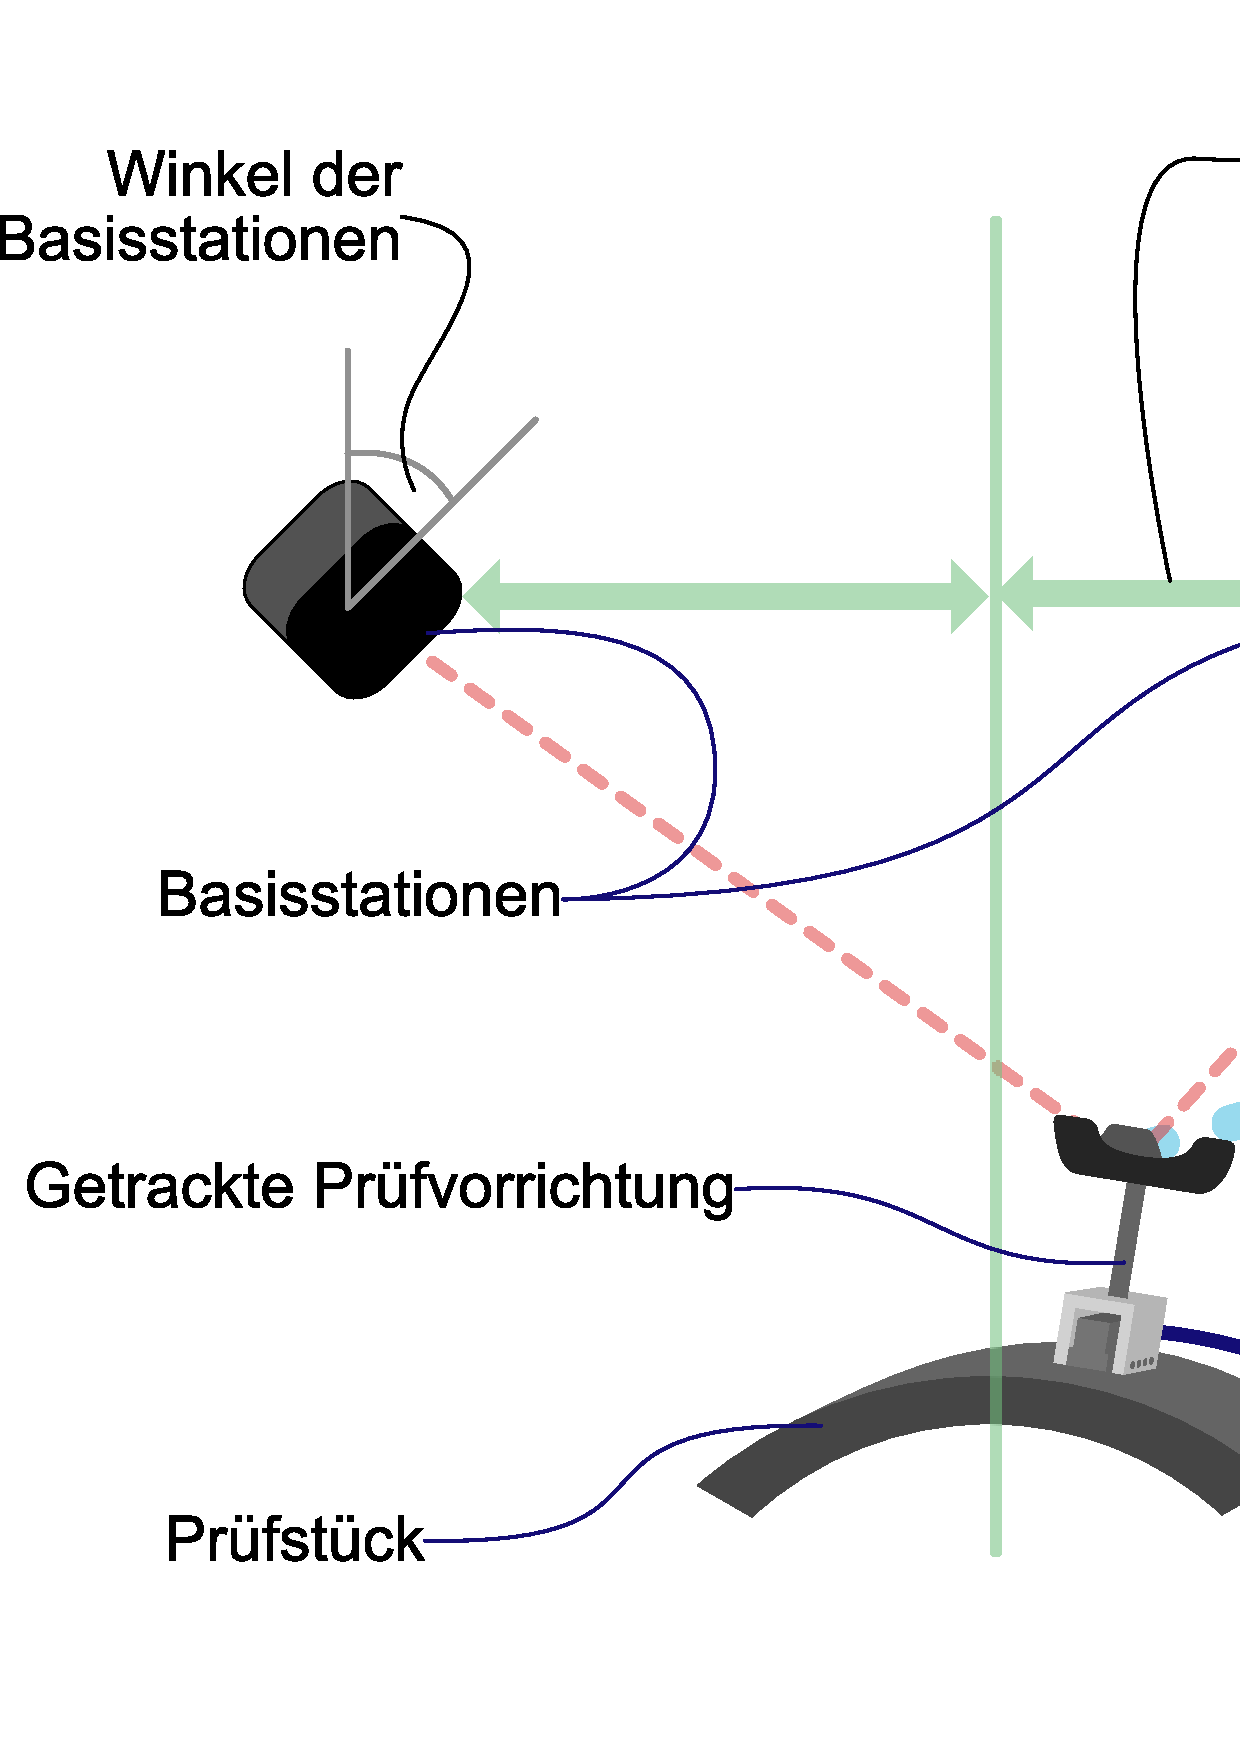
\includegraphics[width=79mm]{images/Setup.pdf}
        \caption{\label{fig:Setup} Setup of the described AR-application. \textcolor{red}{Grafik muss noch übersetzt werden.}}
        % TODO: Grafik übersetzen, ZEDmini hinzufügen
    \end{center}
\end{figure}

\subsection{Tracking of the ultrasonic probe}
The ultrasonic probe is tracked with the help of a attachable tracked \textit{VIVE}--Tracker.
This Tracker is attached to a mount, in which the ultrasonic probe is fixed (figure~\ref{fig:probemount}).
The offset and orientation between the tracker and probe is applied in software by setting the virtual probe as a child transform of the tracker.

\begin{figure}[h!]
  \label{fig:probemount}
    \begin{center}
        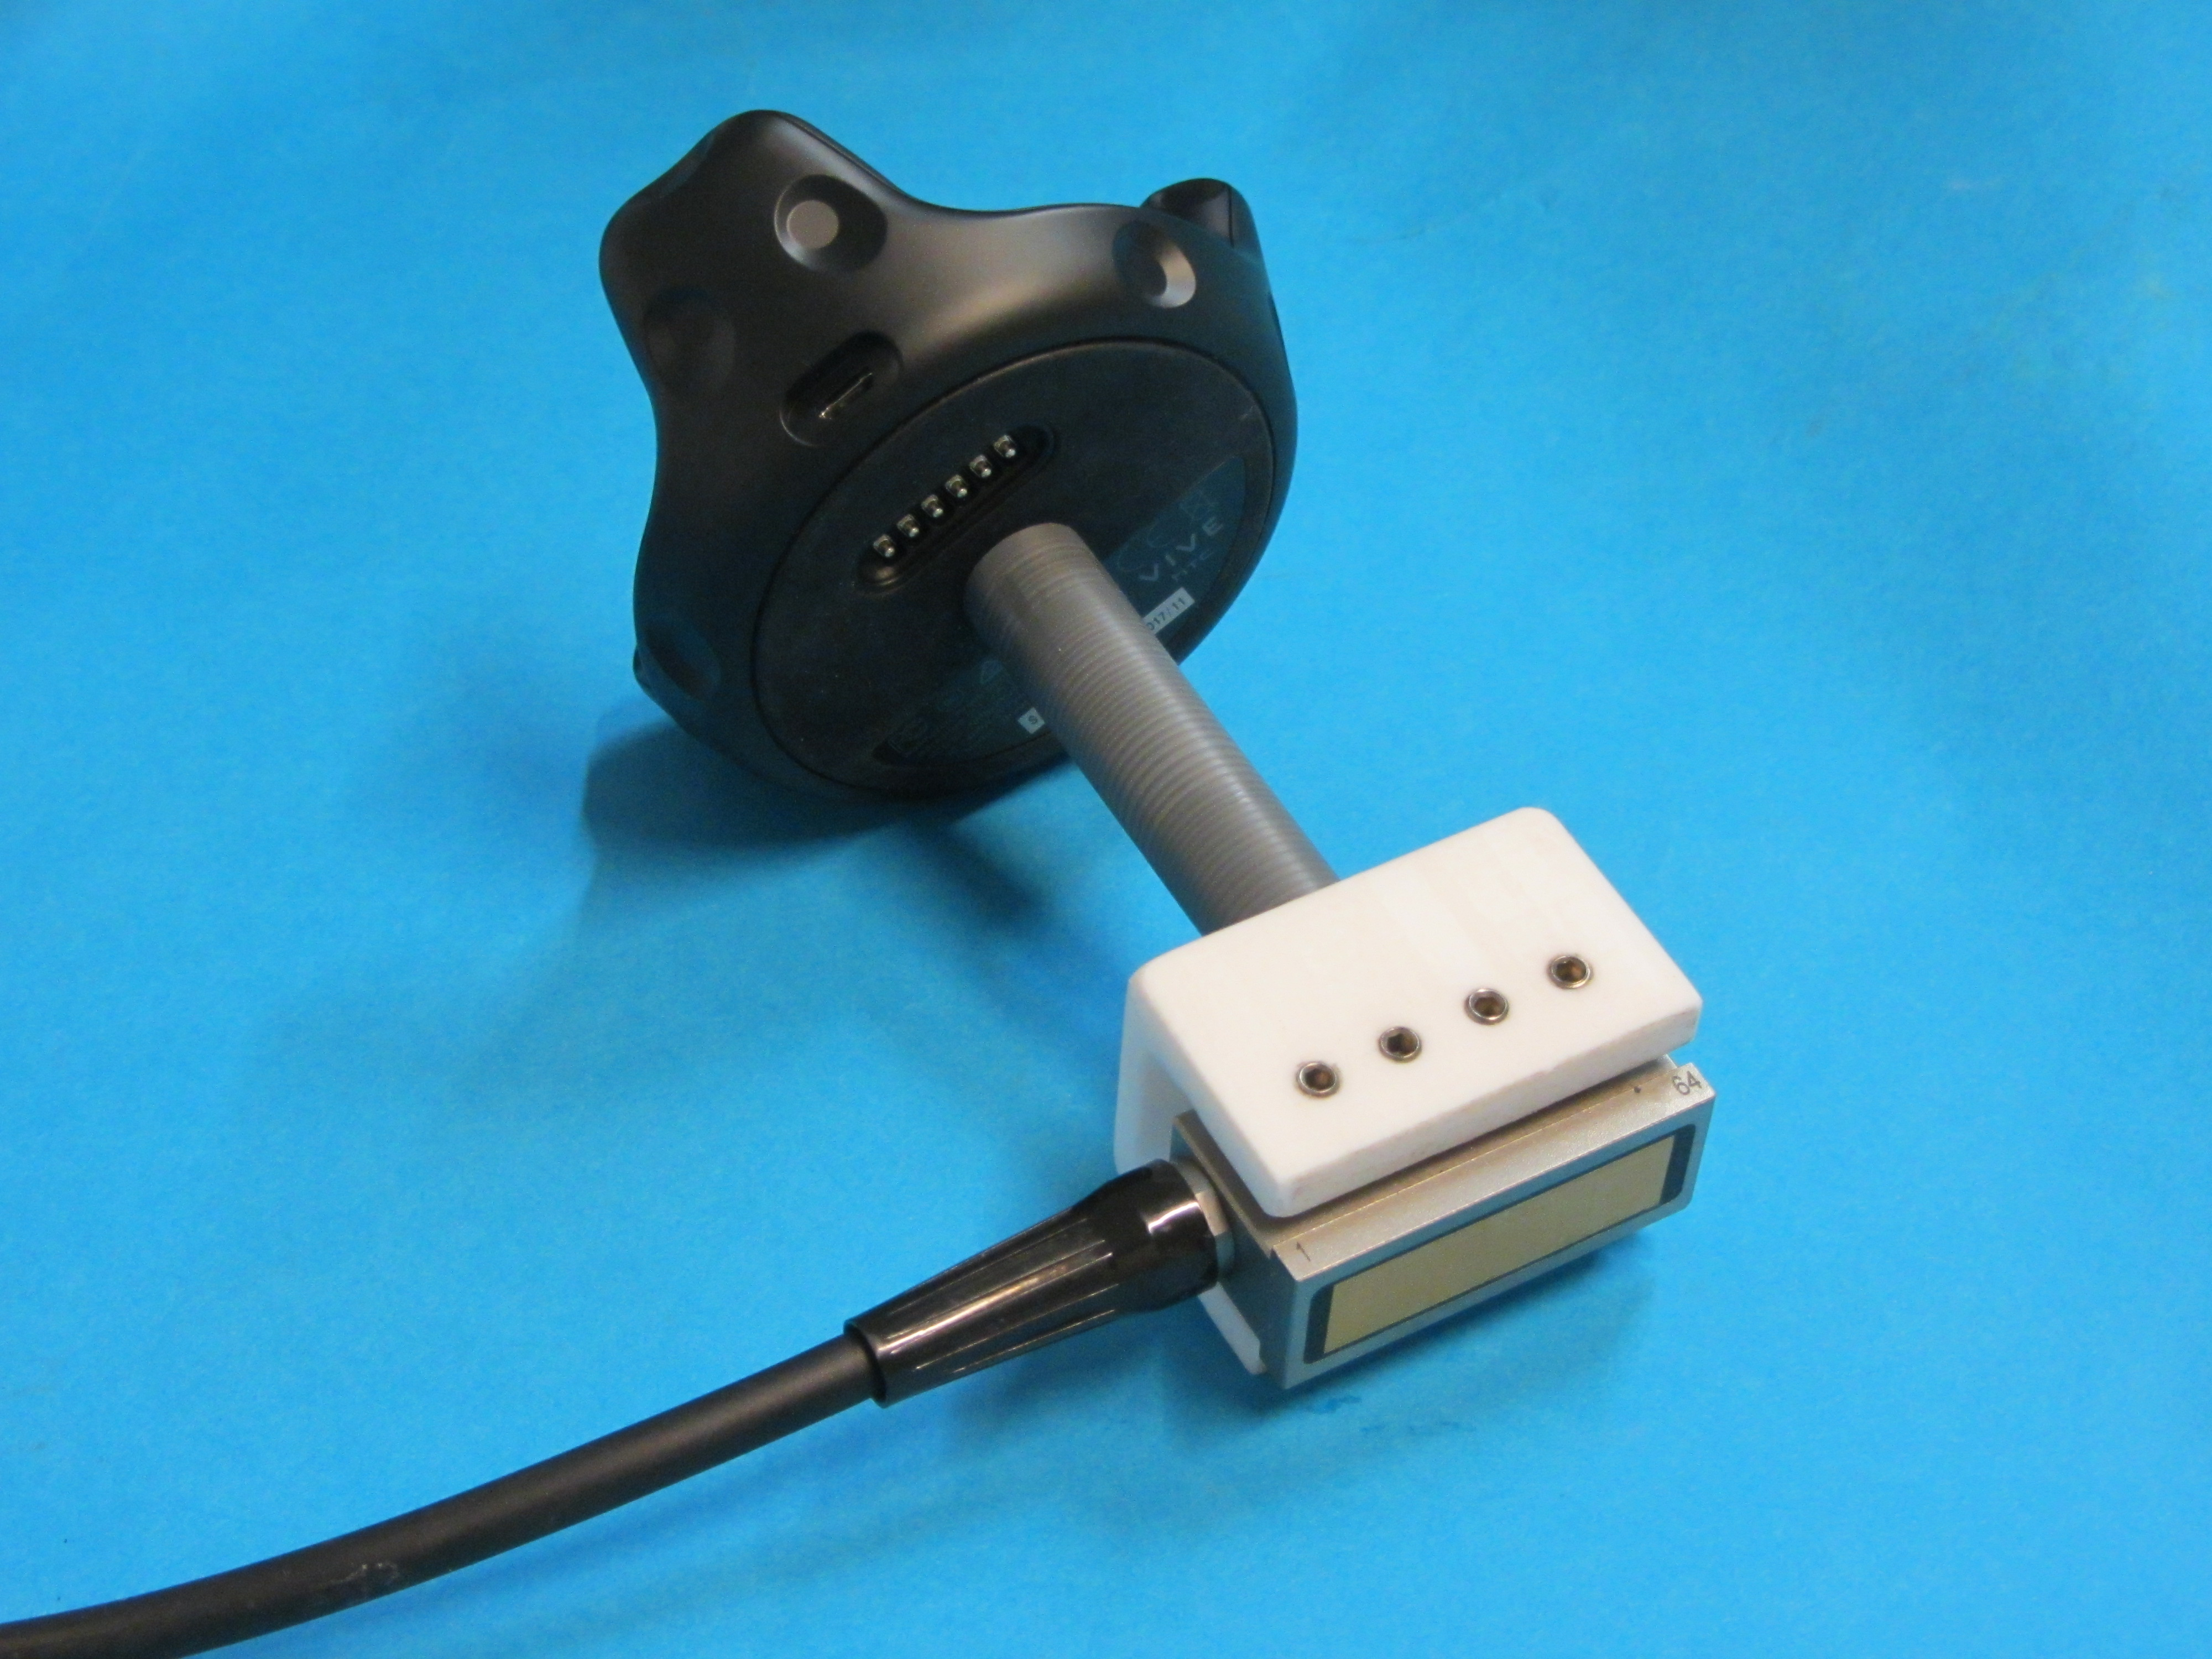
\includegraphics[width=79mm]{images/probemount.jpg}
        \caption{\label{fig:probemount} Probemount, that fixes \textit{VIVE--}Tracker to ultrasonic probe.}
    \end{center}
\end{figure}

\subsection{Detection of the coordinate system in worldspace}
The coordinate system of the surface to be measured is detected in two steps:
first a point--cloud of the surface is created by moving the tracked probe across it.
In the next step the parameters of the selected geometry in worldspace are calculated from this point--cloud using the Downhill--Simplex optimization by Nelder and Mead.
In a second step the used coordinate system is picked by placing the tracked probe at the desired origin and pressing the setup button.
As the specimen--geometry is already defined, only one more axis is required to define the orthogonal coordinate system.
this is done by placing the tracked probe on the X--Axis and pressing the setup button.

\subsection{Vizualisation of the tracking--data}

\begin{figure}[h!]
    \begin{center}
        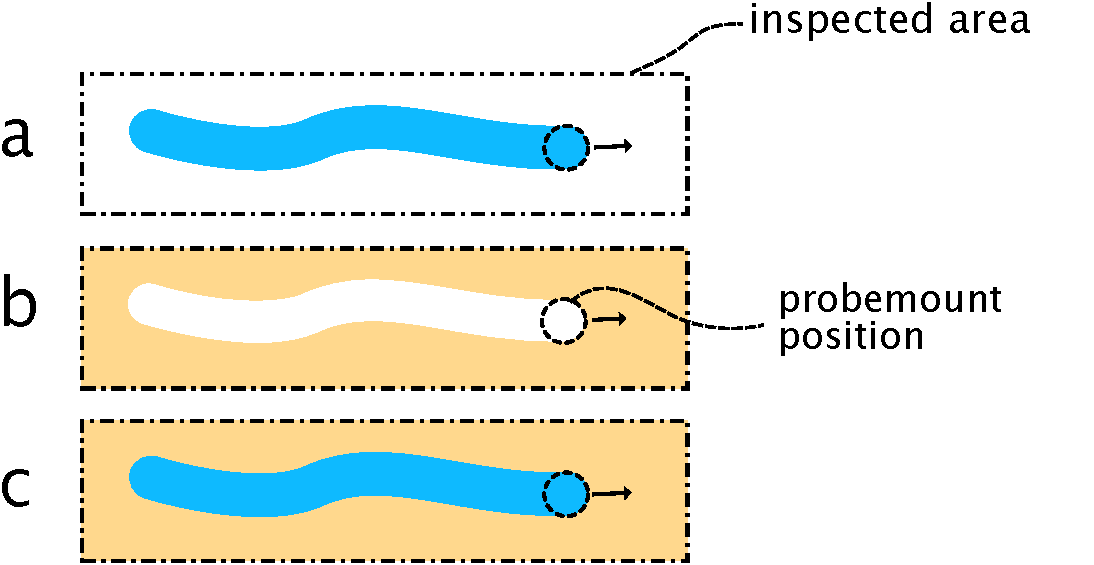
\includegraphics[width=79mm]{images/DrawVsErase.pdf}
        \caption{\label{fig:DrawVsErase} Different methods to mark covered area.}
    \end{center}
\end{figure}

\subsection{Continuous and singular logging of position}

\section{Evaluation of the \textit{VIVE}--tracker accuracy}
The accuracy of the \textit{VIVE}--Tracker was determined in a experiment using an automated X--Y--scanner.
Both \textit{VIVE}--Basestations were positioned on opposite corners of the scanner, though one at a greater distance (figure~\ref{fig:precisionMeasurementSetup}).

\begin{figure}[h!]
    \begin{center}
        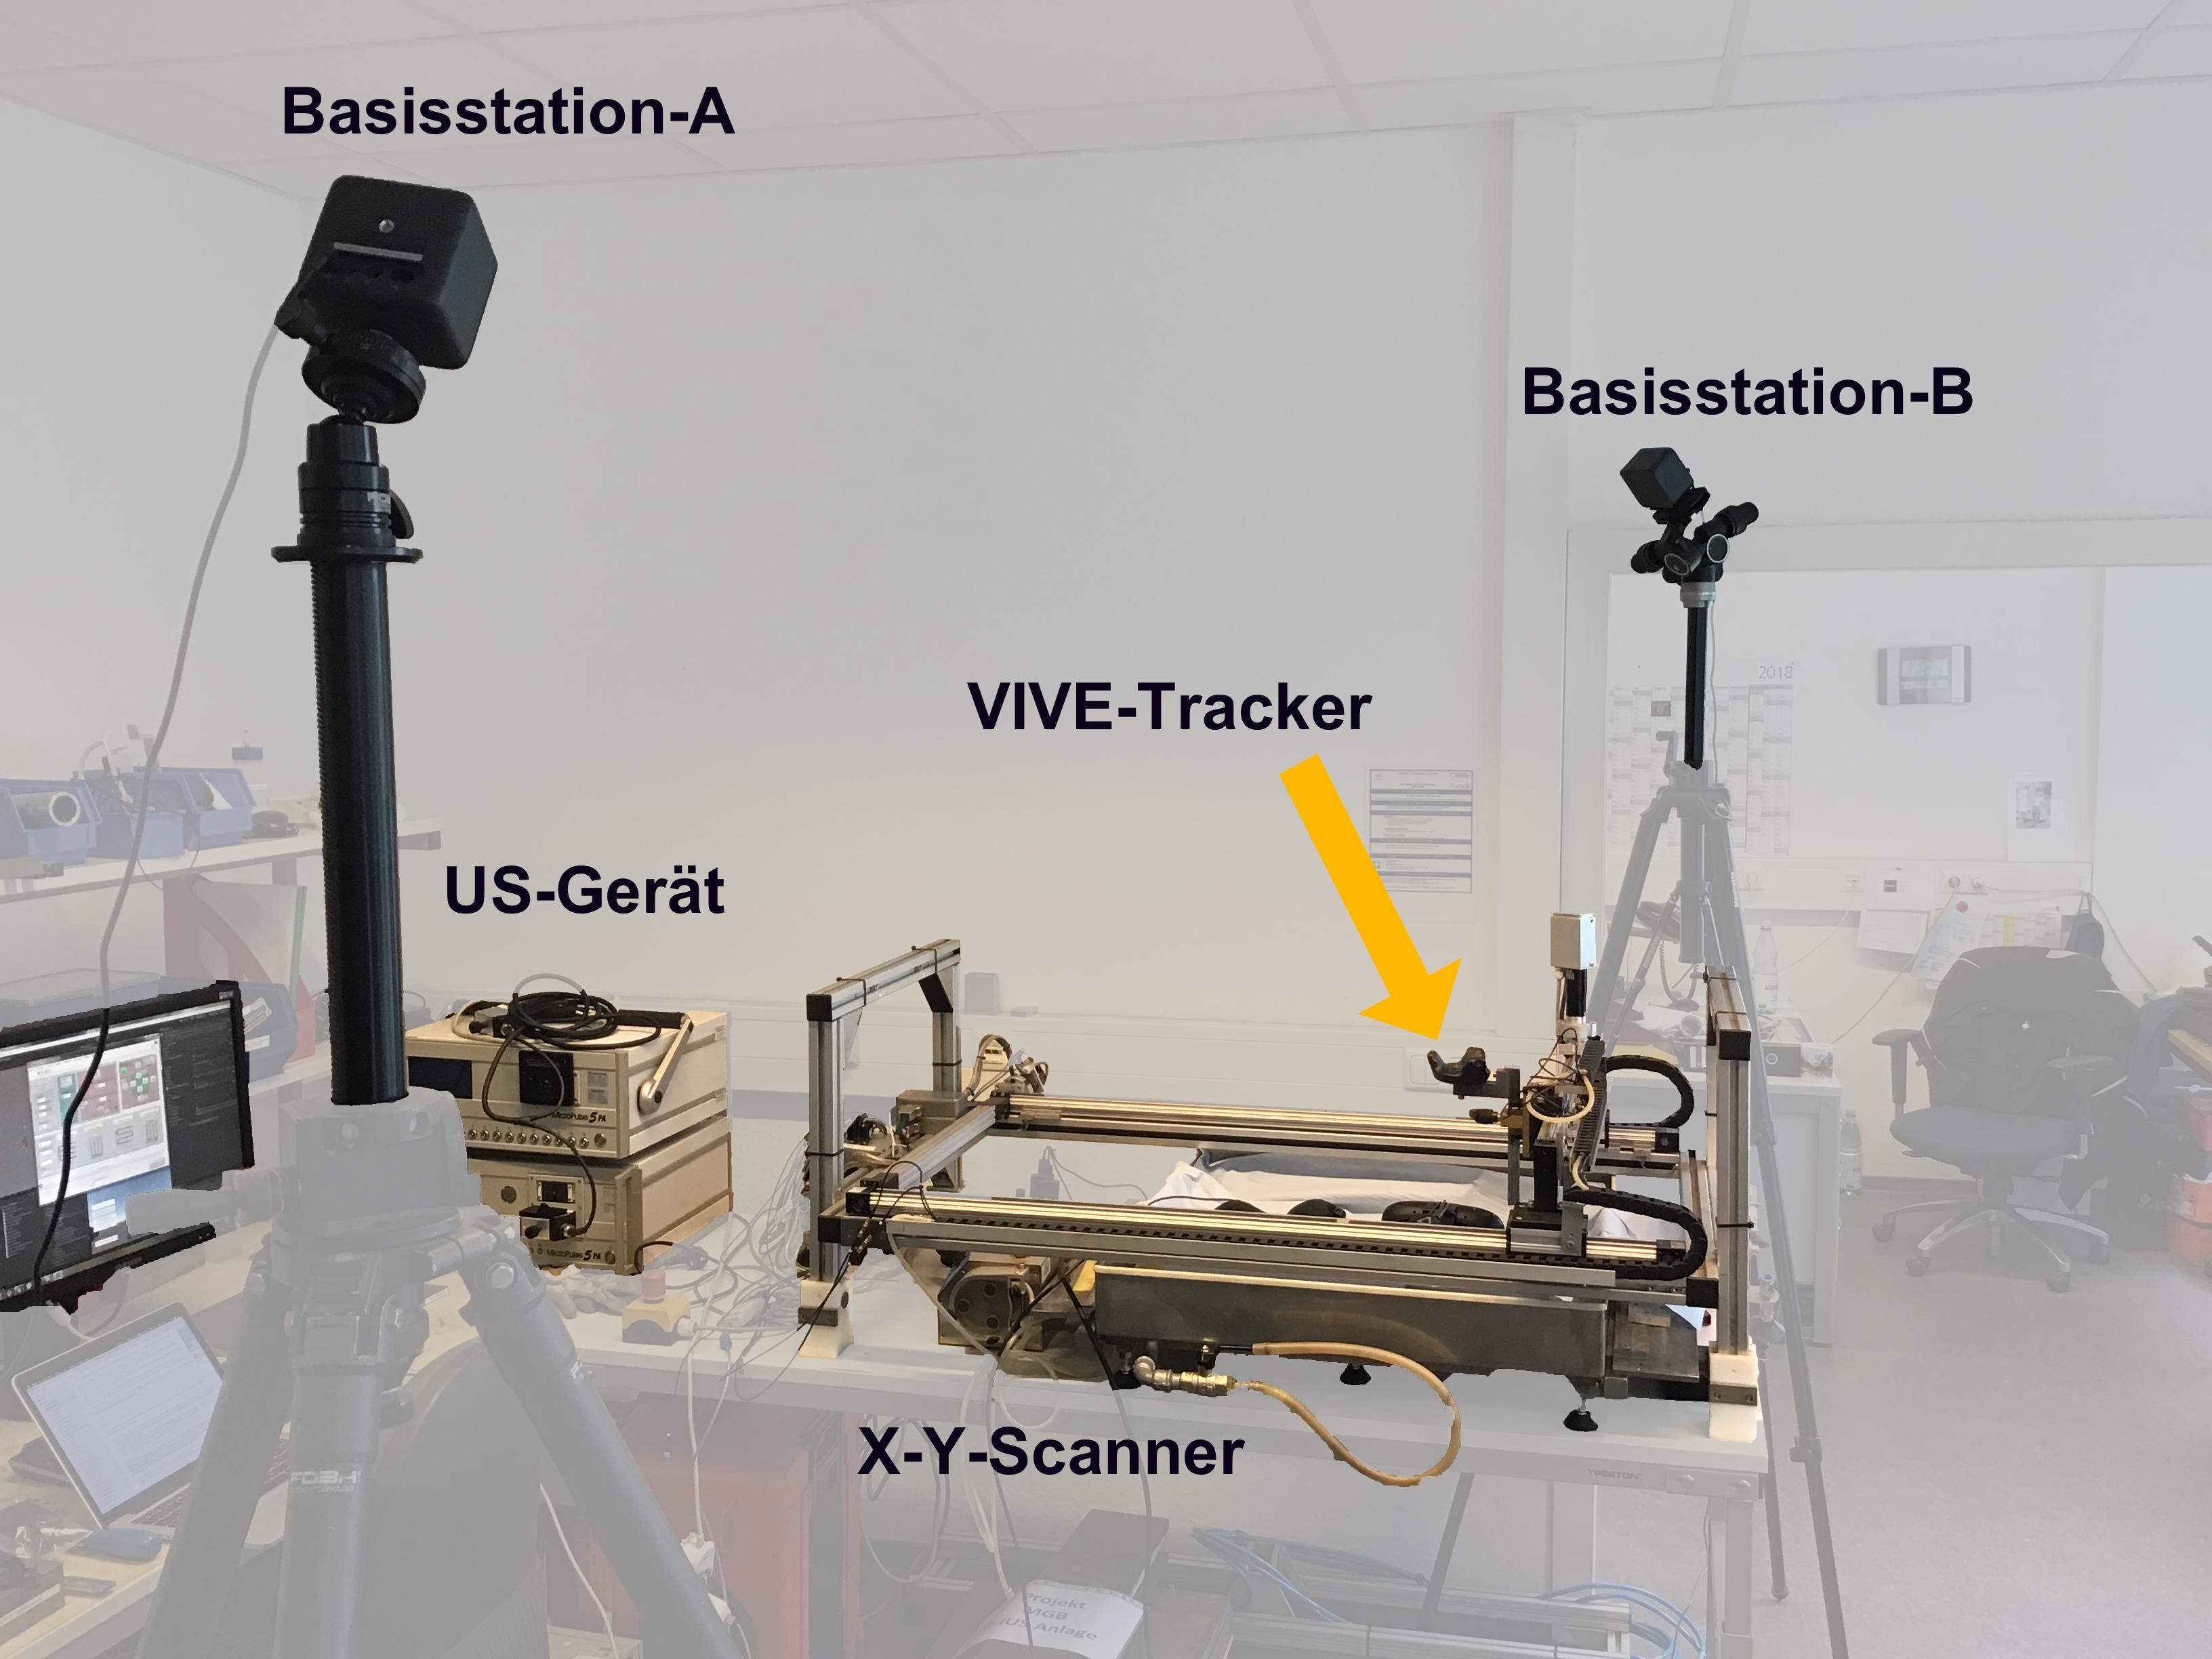
\includegraphics[width=79mm]{images/PrecisionMeasurement.jpg}
        \caption{\label{fig:precisionMeasurementSetup} Setup for the evaluation of the \textit{VIVE}--Precision. \textcolor{red}{Grafik muss noch übersetzt werden.}}
    \end{center}
\end{figure}

The tracker was screwed to the moving head of the scanner and moved in a comb structure over a surface of 400\,mm x 800\,mm.
During the process, the position of the tracker and absolute time was continuously logged.
In the beginning and end of each comb tine the movement was paused by 2\,s to identify the position in the log--file.\\

The evaluation was done by choosing the start position as a reference and calculating the difference between the distance of the measured and the calculated position to it.
These differences are plottet subject to the tine and type of comb.

\begin{figure}[h!]
    \begin{center}
        
\includegraphics[width=79mm]{images/distancesBoxplot-E.pdf}
        \caption{\label{fig:boxplotE} Difference between measured and theoretical distances to the reference point at the E--Positions.}
    \end{center}
\end{figure}

\begin{figure}[h!]
    \begin{center}
        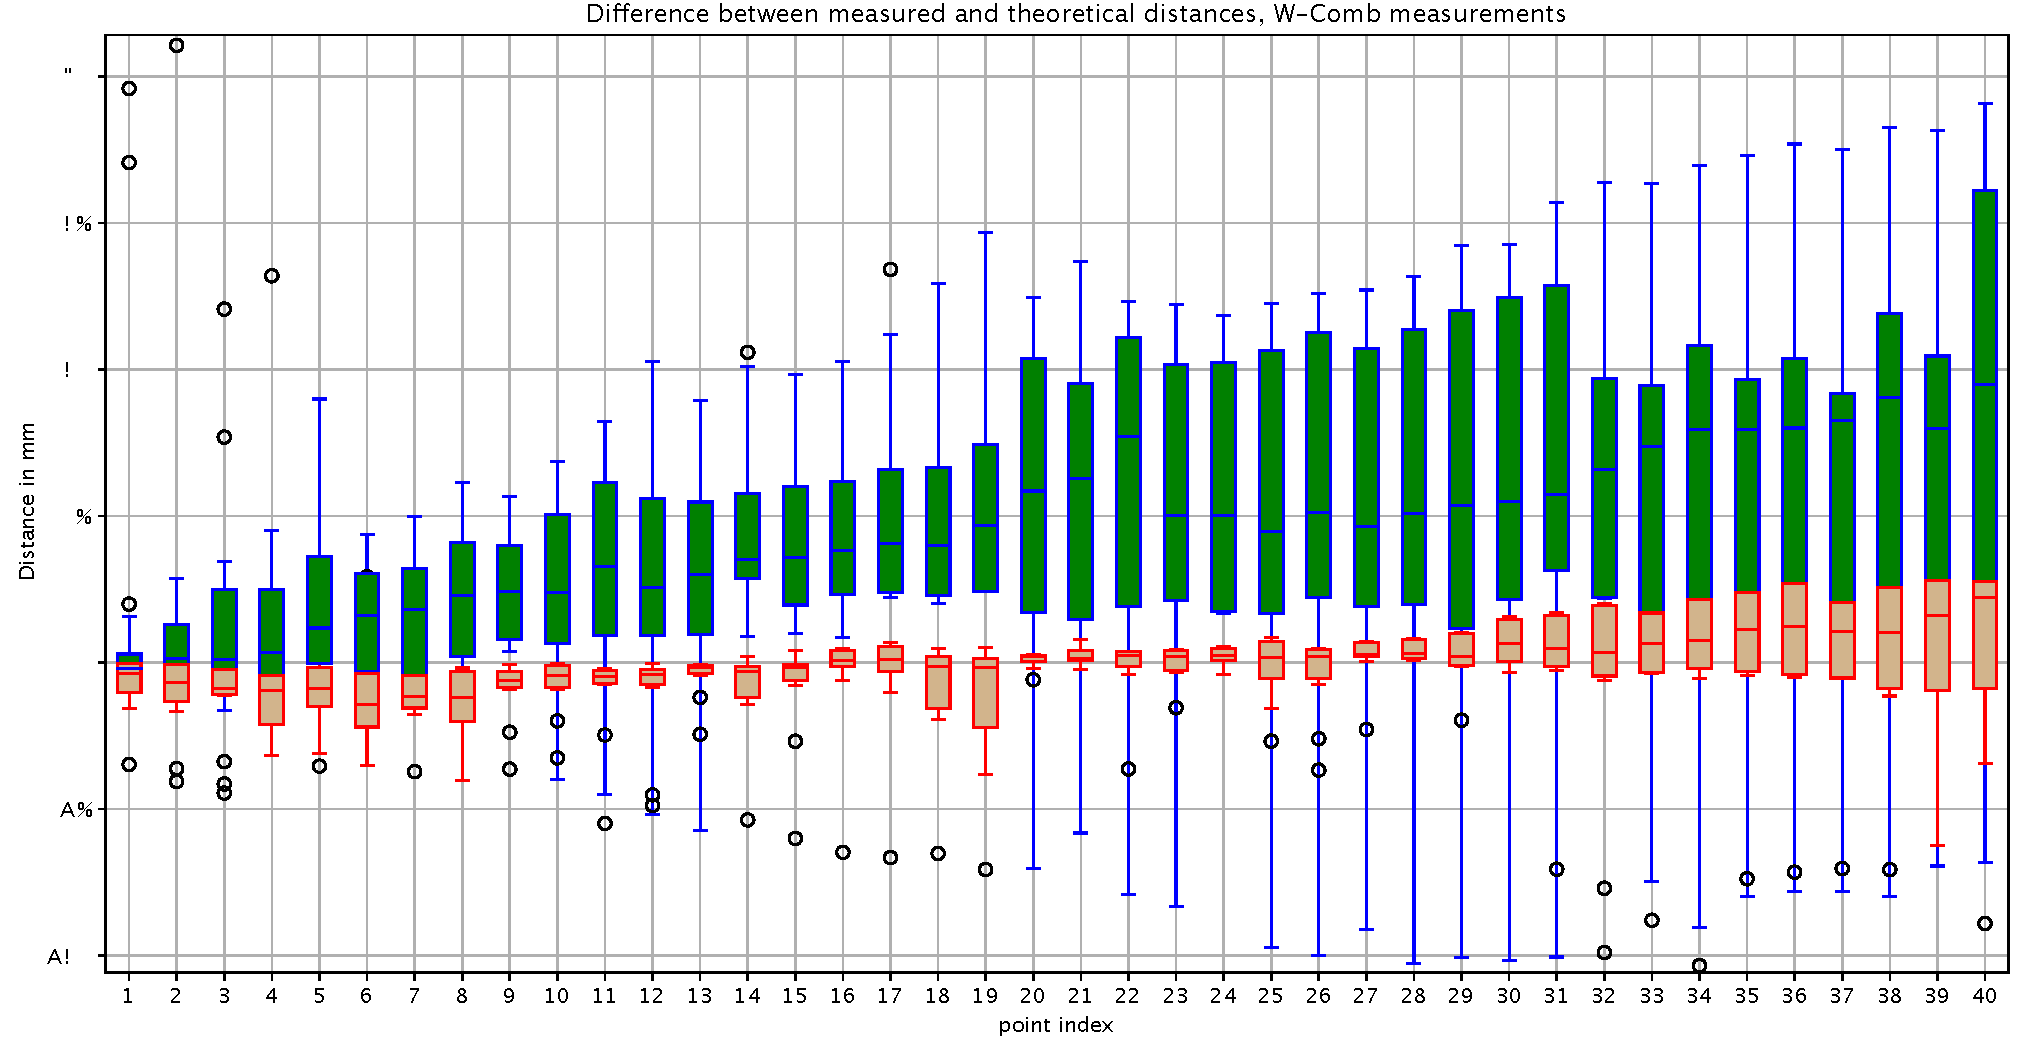
\includegraphics[width=79mm]{images/distancesBoxplot-W.pdf}
        \caption{\label{fig:boxplotW} Difference between measured and theoretical distances to the reference point at the W--Positions.}
    \end{center}
\end{figure}

The results show a decline in quality as the surveypoints get closer to the closer basestation (basestation--B in figure~\ref{fig:precisionMeasurementSetup}) with an error up to 18\,mm.
In the opposite corner the values had a quality of about 1--2\,mm.
This can be explained by the rapidly declining quality as the proximity to the basestation is too small.

\section{Conclusion}

\begin{figure}[h!]
    \begin{center}
        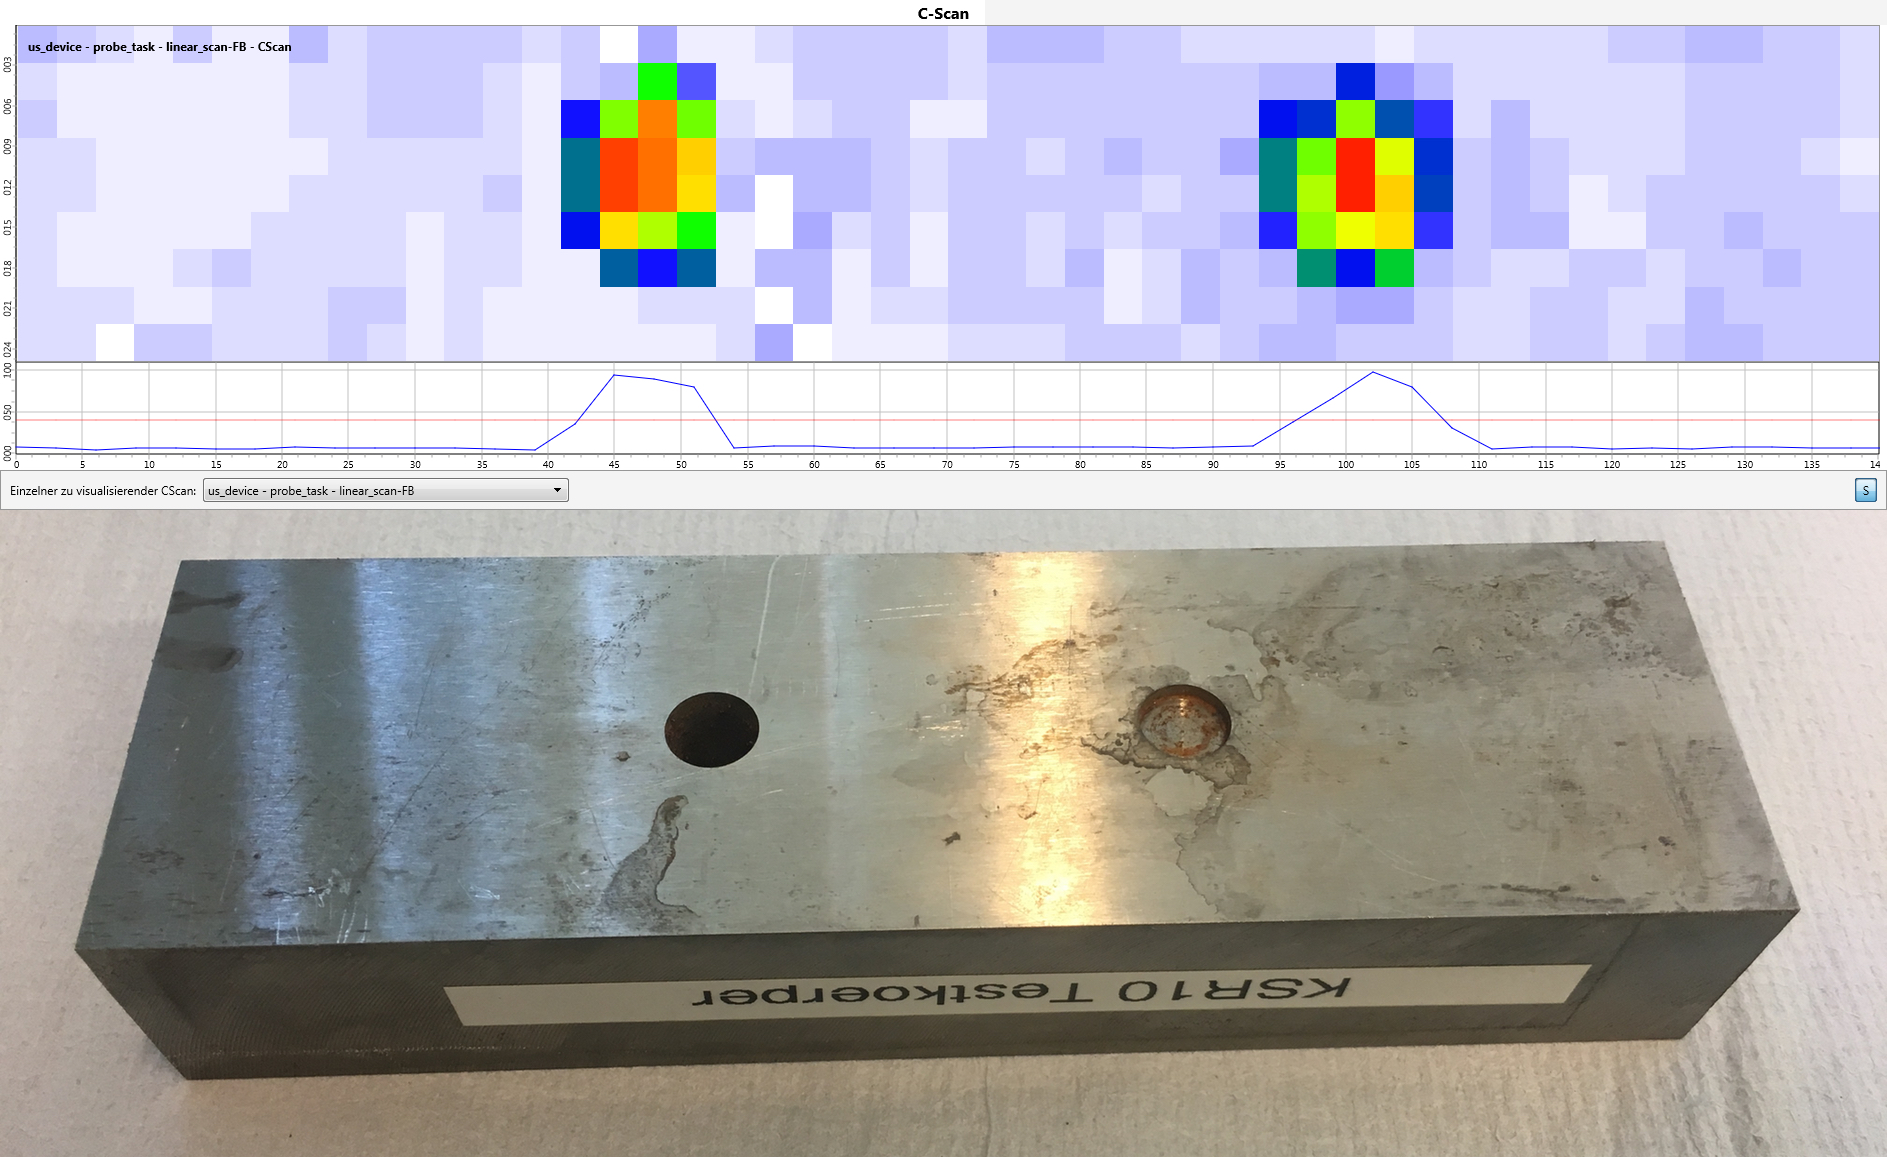
\includegraphics[width=79mm]{images/CScanARUS.jpg}
        \caption{\label{fig:resultCScan} Mit Hilfe des Tracking Systems erstellter C--Scan}
    \end{center}
\end{figure}

\VRARsetbibstyle
\bibliography{VRARTeXample}

\end{document}
